% ==========================================
% EINLEITUNG
% ==========================================
\chapter{Einleitung}

\section{Projektumfeld}

\subsection{Unternehmen}
Die EDAG Engineering GmbH ist ein international tätiger Engineering-Dienstleister mit Hauptsitz in Wiesbaden, Deutschland. Als einer der weltweit führenden unabhängigen Engineering-Partner entwickelt EDAG innovative Lösungen für die Automobilindustrie und weitere Mobilitätsbranchen\cite{edag_unternehmen}. Das 1969 gegründete Unternehmen beschäftigt mehrere tausend Mitarbeiter an über 80 Standorten weltweit und erwirtschaftet einen Jahresumsatz im hohen dreistelligen Millionen-Euro-Bereich\cite{edag_zahlen}.

\subsection{Abteilung}
Das Projekt wird in der Abteilung \textit{Mobility IT} durchgeführt, die innovative Softwarelösungen für Smart City und Automotive-Projekte entwickelt. Das interdisziplinäre Team besteht aus knapp 100 Mitarbeitern mit unterschiedlichen Kompetenzen in den Bereichen \gls{frontend}- und \gls{backend}-Entwicklung, \gls{devops}, Cloud-Architektur und Projektmanagement. Die Abteilung arbeitet mit modernen Cloud-Native-Technologien wie Docker\cite{docker_docs} und Kubernetes\cite{kubernetes_docs}, agilen Methoden (\gls{scrum}, \gls{kanban}) und \gls{devops}-Praktiken\cite{agile_manifesto,devops_what_is}. Das im Rahmen dieser Projektarbeit entwickelte Skill-Management-System ist als internes Tool konzipiert und soll die Ressourcenplanung innerhalb der Abteilung optimieren.

\section{Ist-Analyse}

Die Personalauswahl für Kundenprojekte erfolgt derzeit durch manuelle, dezentrale Prozesse ohne zentrale Kompetenzübersicht. Projektmanager nutzen veraltete Excel-Tabellen und führen zeitaufwendige E-Mail-Anfragen bei Teamleitern durch, um geeignete Mitarbeiter zu identifizieren.

\subsection{Probleme des aktuellen Prozesses}
\begin{itemize}
    \item Fehlende zentrale, aktuelle Übersicht über Mitarbeiterkompetenzen und deren Ausprägung
    \item Zeitaufwendige Suche nach geeigneten Mitarbeitern (durchschnittlich 2,5 Stunden pro Projektbesetzung\cite{projektbesetzung_aufwand})
    \item Keine systematische, nachvollziehbare Dokumentation von \glspl{skill} und Projekterfahrungen
    \item Erhöhtes Risiko von Fehlbesetzungen durch unvollständige oder veraltete Informationen
    \item Ineffiziente Ressourcennutzung und potenzielle Überlastung einzelner Mitarbeiter
    \item Mangelnde Transparenz über verfügbare Kompetenzen behindert strategische Personalentwicklung
\end{itemize}

\subsection{Wirtschaftliche Auswirkungen}
Bei 50 Projektbesetzungen jährlich entstehen Opportunitätskosten von 9.375\,€ (125 Stunden × 75\,€/h)\cite{projektbesetzung_aufwand,projektleiter_stundensatz}. Die detaillierte Wirtschaftlichkeitsbetrachtung erfolgt in Kapitel~\ref{sec:wirtschaftlichkeit}.

\section{Zielsetzung}

Das Ziel ist die Entwicklung eines webbasierten Skill-Management-Systems als \gls{mvp}, das eine effiziente, datenbasierte Personalauswahl ermöglicht und die Transparenz über Mitarbeiterkompetenzen erhöht. Der \gls{mvp}-Ansatz fokussiert auf die Kernfunktionalitäten, die den größten Mehrwert für die Abteilung liefern, und ermöglicht eine schnelle Inbetriebnahme mit späteren Erweiterungsmöglichkeiten.

\subsection{Funktionale Anforderungen}

Das \gls{mvp} unterstützt drei Benutzerrollen mit unterschiedlichen Berechtigungen:

\paragraph{Mitarbeiter (Employee):}
\begin{itemize}
    \item Personalisiertes Dashboard mit Übersicht über Skill-Entwicklung, zugewiesene Projekte und relevante Kennzahlen
    \item Umfassende Profilverwaltung: \glspl{skill} mit Selbsteinschätzung (Skala 0--100), persönliche Beschreibung, Berufserfahrung und Verfügbarkeit
    \item Suchfunktion für Mitarbeiter
    \item Übersicht über eigene Projektzuordnungen und kürzliche Aktivitäten im System
\end{itemize}

\paragraph{Projektleiter (Manager):}
\begin{itemize}
    \item Alle Funktionen der Mitarbeiter-Rolle
    \item Projektmanagement: Projekte anlegen, bearbeiten und Teams zusammenstellen
    \item Projektsuche mit Filtern nach \glspl{skill}, Mitarbeiterzuordnungen und Projektstatus
\end{itemize}

\paragraph{Administrator (Admin):}
\begin{itemize}
    \item Alle Funktionen der Mitarbeiter-Rolle
    \item Benutzerverwaltung: Rollenzuweisung (Admin, Manager, Mitarbeiter), Bearbeitung von Rollenanfragen
    \item Stammdatenverwaltung: Pflege von \glspl{skill}, Skill-Kategorien, Standorten und Positionen
\end{itemize}

\subsection{Nicht-funktionale Anforderungen}
\label{sec:nicht_funktionale_anforderungen}
\begin{itemize}
    \item \textbf{Usability:} Intuitive Benutzeroberfläche ohne Schulungsaufwand, konform zu Usability-Standards\cite{wcag}
    \item \textbf{Performance:} Antwortzeiten unter 2 Sekunden für Suchanfragen, maximale Seitenladezeit von 3 Sekunden\cite{web_performance}
    \item \textbf{Sicherheit:} Sichere Authentifizierung über \gls{oauth} 2.0 und \gls{oidc} mit Keycloak\cite{keycloak_docs}, rollenbasierte Zugriffskontrolle\cite{oauth2_spec}
    \item \textbf{Skalierbarkeit:} Architektur für unternehmensweiten Einsatz mit mehreren hundert Benutzern ausgelegt mittels Kubernetes\cite{kubernetes_docs}
    \item \textbf{Wartbarkeit:} Modulare Architektur nach \gls{clean_architecture}-Prinzipien, Code-Qualitätssicherung\cite{clean_architecture}
    \item \textbf{Integration:} Automatische Synchronisation von Benutzerdaten aus Keycloak\cite{keycloak_docs}, Api-First-Ansatz für zukünftige Integrationen\cite{api_design}
\end{itemize}

\subsection{Use-Case-Übersicht}

Abbildung~\ref{fig:use_case_overview} zeigt die Hauptfunktionen des Systems und deren Zuordnung zu den drei Benutzerrollen gemäß \gls{uml}-Standard\cite{uml_specification}.

\begin{figure}[H]
\centering
\begin{tikzpicture}[
    scale=1.0,
    every node/.style={transform shape},
    actor/.style={},
    usecase/.style={ellipse, draw, minimum width=2.5cm, minimum height=0.8cm, font=\small, align=center},
    include/.style={->, dashed, font=\scriptsize},
    extends/.style={->, dashed, font=\scriptsize}
]

% Akteure links
\node[font=\small] (employee) at (-3.5, 0) {
    \begin{tikzpicture}
        \draw[thick] (0,0.3) circle (0.12cm);
        \draw[thick] (0,0.1) -- (0,-0.2);
        \draw[thick] (0,0) -- (-0.15,-0.2);
        \draw[thick] (0,0) -- (0.15,-0.2);
        \draw[thick] (0,-0.2) -- (-0.1,-0.45);
        \draw[thick] (0,-0.2) -- (0.1,-0.45);
    \end{tikzpicture}
};
\node[below=0.2cm of employee, font=\small] {Mitarbeiter};

\node[font=\small] (manager) at (-3.5, 5) {
    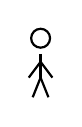
\begin{tikzpicture}
        \draw[thick] (0,0.3) circle (0.12cm);
        \draw[thick] (0,0.1) -- (0,-0.2);
        \draw[thick] (0,0) -- (-0.15,-0.2);
        \draw[thick] (0,0) -- (0.15,-0.2);
        \draw[thick] (0,-0.2) -- (-0.1,-0.45);
        \draw[thick] (0,-0.2) -- (0.1,-0.45);
    \end{tikzpicture}
};
\node[below=0.2cm of manager, font=\small] {Projektleiter};

\node[font=\small] (admin) at (-3.5, -5) {
    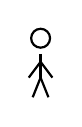
\begin{tikzpicture}
        \draw[thick] (0,0.3) circle (0.12cm);
        \draw[thick] (0,0.1) -- (0,-0.2);
        \draw[thick] (0,0) -- (-0.15,-0.2);
        \draw[thick] (0,0) -- (0.15,-0.2);
        \draw[thick] (0,-0.2) -- (-0.1,-0.45);
        \draw[thick] (0,-0.2) -- (0.1,-0.45);
    \end{tikzpicture}
};
\node[below=0.2cm of admin, font=\small] {Administrator};

% System-Boundary - größer für bessere Verteilung
\draw[thick, rounded corners=8pt] (-0.5, -7) rectangle (10.5, 7);
\node[above right, font=\small] at (-0.5, 7) {\texttt{<<system>>}};
\node[above, font=\bfseries] at (5, 7) {Skill Management System};

% Use Cases - Mitarbeiter (Mitte) - gleichmäßiger verteilt
\node[usecase] (profil) at (2, 2.5) {Profil\\verwalten};
\node[usecase] (skills) at (9, -2) {Skills\\bearbeiten};
\node[usecase] (dashboard) at (6, 2) {Dashboard\\anzeigen};
\node[usecase] (suche) at (5.5, -0.5) {Mitarbeiter\\suchen};
\node[usecase] (projekte) at (8.5, 0.5) {Projekte\\durchsuchen};
\node[usecase] (rollenanfrage) at (2, -2) {Rollenanfrage\\stellen};

% Use Cases - Manager (oben) - gleichmäßiger verteilt
\node[usecase] (projekt) at (2, 6) {Projekt\\erstellen};
\node[usecase] (team) at (8, 5.3) {Team\\zusammenstellen};
\node[usecase] (filter) at (2.5, 4) {Skills\\filtern};
\node[usecase] (verfuegbar) at (8.5, 3) {Verfügbarkeit\\prüfen};

% Use Cases - Admin (unten) - gleichmäßiger verteilt
\node[usecase] (benutzer) at (1, -3.4) {Benutzer\\verwalten};
\node[usecase] (stammdaten) at (5.5, -3.5) {Stammdaten\\verwalten};
\node[usecase] (rollen) at (5.5, -6) {Rollen\\zuweisen};
\node[usecase] (anfragepruef) at (8.5, -4.5) {Rollenanfragen\\prüfen};

% Generalisierung zwischen Akteuren
\draw[-{Triangle[length=3mm, width=2.5mm, fill=white]}, thick] (manager) -- (employee);
\draw[-{Triangle[length=3mm, width=2.5mm, fill=white]}, thick] (admin) -- (employee);

% Assoziationen - Mitarbeiter
\draw[-] (employee) -- (profil);
\draw[-] (employee) -- (skills);
\draw[-] (employee) -- (dashboard);
\draw[-] (employee) -- (suche);
\draw[-] (employee) -- (projekte);
\draw[-] (employee) -- (rollenanfrage);

% Assoziationen - Manager (nur exklusive)
\draw[-] (manager) -- (projekt);
\draw[-] (manager) -- (team);
\draw[-] (manager) -- (filter);

% Assoziationen - Admin (nur exklusive)
\draw[-] (admin) -- (benutzer);
\draw[-] (admin) -- (stammdaten);
\draw[-] (admin) -- (rollen);
\draw[-] (admin) -- (anfragepruef);

% Include-Beziehungen (gestrichelt)
\draw[include] (skills) -- (stammdaten)
    node[pos=0.5, sloped, font=\scriptsize, xshift=6pt, yshift=-4pt]{<<include>>};
\draw[include]
    (projekt)
    to[out=-20, in=140]
    node[midway, below, sloped, font=\scriptsize]{<<include>>}
    (suche);
\draw[include] (team) -- (filter) node[midway, above, font=\scriptsize] {<<include>>};

% Extends-Beziehungen (gestrichelt)
\draw[extends] (verfuegbar) -- (filter) node[midway, right, font=\scriptsize] {<<extends>>};
\draw[extends]
    (rollen)
    to[out=45, in=-135]
    node[midway, above, sloped, font=\scriptsize]{<<extends>>}
    (anfragepruef);

\end{tikzpicture}
\caption{Use-Case-Diagramm des Skill Management Systems}
\label{fig:use_case_overview}
\end{figure}

Das System nutzt Keycloak\cite{keycloak_docs} als zentralen \gls{idp}, wodurch die Implementierung vereinfacht wird und eine spätere Integration in das unternehmensweite \gls{sso} der EDAG ermöglicht wird. Alle im Use-Case-Diagramm dargestellten Aktionen setzen zudem eine erfolgreiche Authentifizierung und rollenbasierte Autorisierung über Keycloak\cite{keycloak_docs} voraus.

\section{Projektnutzen}

Die Automatisierung reduziert den Aufwand pro Projektbesetzung von 2,5 Stunden auf 15 Minuten (90\% Reduktion), was jährlich 8.437,50\,€ einspart (siehe Abschnitt~\ref{sec:nutzen_analyse})\cite{projektbesetzung_aufwand,projektleiter_stundensatz}. Zusätzliche Vorteile:

\begin{itemize}[noitemsep]
    \item Transparente Kompetenzübersicht für strategische Personalplanung
    \item Datenbasierte Personalauswahl verbessert Projekterfolgsrate
    \item Sichtbarkeit individueller Kompetenzen erhöht Mitarbeiterzufriedenheit
    \item Fundierte Grundlage für gezielte Weiterbildungsmaßnahmen
\end{itemize}

\section{Projektabgrenzung}

Das \gls{mvp} ist als internes Tool für die Abteilung Mobility IT konzipiert. Die Architektur unterstützt eine spätere unternehmensweite Ausweitung.

\textbf{Im Projektumfang:} Webbasierte Anwendung mit Skill-/Projektverwaltung, rollenbasiertem Zugriff, Keycloak-Integration und REST-Api.

\textbf{Ausgeschlossen:} Native mobile Apps, HR-System-Integrationen, erweiterte Analytics und Reporting-Funktionen.
